\chapter{Implementacja}

Aplikacja Elements została zaprojektowana w taki sposób, by z łatwością można było ją dopasować do innych składowych systemu ogrzewania rozjazdów kolejowych. W związku z tym, aplikacja przygotowana jest do instalacji na serwerze xsp4 zintegrowanym z apache, przy użyciu maszyny wirtualnej Mono. Wyżej wymienione technologie są kompatybilne z systemami z rodziny Unix, na których działa reszta aplikacji systemu.

\section{Wykorzystane biblioteki}

\subsection{Razor}

Razor jest silnikiem generowania widoków autorstwa Microsoft, który w swojej składni jest znacznie prostszy niż jego poprzednik – aspx. Dzięki temu tworzenie stron, które wymagają użycia logiki staje się jeszcze łatwiejsze. Uproszczenie składni polega głównie na zastąpieniu znaczników aspx jednym znakiem - „@”. Służy on do zadeklarowania w widoku intencji użycia zmiennych dostarczanych do niego przez kontroler. Wydawać by się mogło, że nie jest to duża różnica, lecz w przypadku skomplikowanych konstrukcjach warunkowych łatwo dostrzec przewagę silnika Razor nad aspx. Dla przykładu następującą składnię aspx:

\begin{lstlisting}[language=HTML]
<%if (Model.Length == 0)

       else
 {%>
   <p><%=Model.Item%></p>
<%} %>
\end{lstlisting}
można zastąpić w taki sposób:
\begin{lstlisting}[language=HTML]
@if (Model.Length == 0)
{
        <p>Brak</p>
}
 else
{
        <p>@Model.Item</p>
}
\end{lstlisting}
W widoku można umieścić sekcję zawierającą logikę. W tym celu należy umieścić linie kodu w konstrukcji @\{...\}. Warto jednak nie zapominać o podstawowym założeniu MVC – widok powinien wyświetlać dane, a nie służyć do ich generowania \cite{design-patterns}.
Razor zawiera również prosty mechanizm tworzenia szablonów stron. Dzięki temu ilość kodu w plikach widoków znacznie się zmniejsza, gdyż powtarzalne części strony takie jak menu, czy stopka można wyeksportować do odrębnych plików.

\subsection{NHibernate}
Nhibernate jest biblioteką, która służy do powiązania tabel baz danych na obiekty (Object Related Mapping) \cite{nhibernate-doc}. Dzięki niej możliwe jest posługiwanie się prostymi obiektami, które swoją strukturą odpowiadają odpowiednim tabelom. Dużą zaletą NHibernate w stosunku do innych bibliotek spełniających tę funkcję jest możliwość konfiguracji w kodzie. Skonfigurować w kodzie można zarówno sposób wiązania obiektów z tabelami, jak i samo połączenie z bazą. Najprostszą metodą konfiguracji jest wskazanie, w którym pakiecie znajdują się obiekty, które powinny zostać powiązane z tabelami za pomocą klasy Configuration. Należy jedynie pamiętać, by nazwy obiektów oraz ich pól były identyczne jak odpowiednie nazwy tabel oraz ich kolumn. Dzięki klasie Configuration uzyskujemy dostęp do obiektu typu SessionFactory, który pozwala na otwieranie i zamykanie sesji z bazą danych. 

Kolejną zaletą NHibernate jest możliwość wykorzystania technologii LINQ do wykonywania zapytań. Dzięki temu kod C\# zawierający zapytanie jest bardzo podobny do odpowiadającego mu zapytania SQL i naturalnie opisuje intencje programisty. Na przykład zapytanie SQL o postaci:
\begin{lstlisting}[language=SQL]
SELECT
    Name
FROM
    Device
WHERE
    Id = 1;
\end{lstlisting}
można zapisać w następujący sposób:
\begin{lstlisting}[language=Java]
string name = session.QueryOver<Device>()
    .Where(d => d.Id == 1)
    .Select(d => d.Name)
    .SingleOrDefault<string>();
\end{lstlisting}
Używanie biblioteki opiera się głównie na wykorzystaniu obiektu SessionFactory. Służy on do otwierania połączenia z bazą danych, wykonywania operacji oraz zamykania połączenia. Wszystkimi wymienionymi czynnościami zajmuje się biblioteka, pozwalając programiście skupić się na logice biznesowej programu.

\subsection{jQuery}
jQuery to biblioteka, która pozwala na osiąganie atrakcyjnych efektów wizualnych na stronie WWW niewielkim nakładem pracy programisty. Jak wiadomo z dokumentacji \cite{jquery-doc}, całość wykonana jest w oparciu o technologię JavaScript. Biblioteka jest niezależna od przeglądarki więc programista nie musi dostosowywać kodu do wielu różnych przeglądarek WWW. Korzystanie z biblioteki polega głównie na korzystaniu z obiektu jQuery lub znaku "\$", który jest aliasem do tego obiektu. jQuery umożliwia wybieranie tablicy węzłów DOM strony internetowej, a następnie wykonywanie na nich różnych działań za pomocą języka JavaScript. Wybieranie węzłów wykonuje się wykorzystując selektory języka CSS3. Przykładowe działania to:
\begin{itemize}
\item dodawanie, usuwanie węzłów
\item odczytywanie i modyfikowanie atrybutów i zawartości węzłów
\item modyfikowanie stylu węzłów
\item animacje
\item rozbudowana obsługa zdarzeń takich jak kliknięcie lub przesunięcie kursora nad element
\end{itemize}
Wszystko to można osiągnąc za pomocą kilku linii kodu, na przykład jeśli programista chciałby zmienić kolor tekstu wszystkich węzłów o klasie \textit{red}, wystarczy posłużyć się następującym kodem:
\begin{lstlisting}[language=Java]
$('.red').css('color': 'red')
\end{lstlisting}
Kolejną istotną funkcją jQuery z punktu widzenia mojej aplikacji jest możliwość wykonywania zapytań synchronicznych jak i asynchronicznych AJAX. Znacznie przyspiesza to tworzenie aplikacji, gdyż różne przeglądarki wymagają obsługi wyżej wymienionych zapytań na różne sposoby. 

W internecie dostępnych jest wiele wtyczek do biblioteki, które rozszerzają funkcjonalność jQuery. Dzięki nim można na przykład w szybki sposób tworzyć interaktywne tabele z danymi (DataTables), przybornik do wyboru koloru (Evol), czy efektywny pokaz slajdów (Fotorama).

\section{Architektura aplikacji}
Zastosowane rozwiązane zostało zaimplementowane jako aplikacja internetowa. Moduł Viewer ma za zadanie wyświetlanie stanu urządzeń w przeglądarce internetowej. Drugi z modułów służy do projektowania tych widoków. Aby maksymalnie ułatwić użytkownikowi tę czynność, moduł Designer został zrealizowany w ten sam sposób. Dzięki temu projektant widoków ma natychmiastową możliwość oceny rezultatów swojej interakcji z aplikacją. Aplikacja została nazwana ,,Elements''. Nawiązuje to do małych elementów, z których budowane są widoki. 

Architektura projektu Elements składa się z trzech warstw zgodnie z ideą wzorca projektowego MVC. Jest to wymuszone przez framework ASP.NET MVC4. 

\subsection{Warstwa prezentacji - Widoki}
Warstwą prezentacji (View) jest interfejs graficzny modułów Designer oraz Viewer. Został on wykonany w dwóch technologiach. Strony internetowe budowane są za pomocą silnika tworzenia widoków Razor. Widoki te zawierają również logikę napisaną w języku TypeScript, który kompiluje się do kodu Javascript. Dzięki temu połączeniu użytkownik jest w stanie poruszać się po interfejsie aplikacji w płynny sposób. Nie ma konieczności przeładowywania formularza na stronach z każdą jego akcją dzięki zastosowaniu zapytań asynchronicznych AJAX. Właśnie na nich oparty w większości jest moduł Viewer. Moduł regularnie wysyła zapytania asynchroniczne do serwera aplikacji w celu pozyskania aktualnych zmiennych. W ten sposób osiągnięty został efekt monitorowania urządzeń w czasie rzeczywistym.

\begin{figure}[h]
	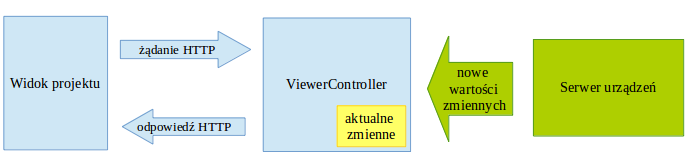
\includegraphics[width=150mm]{./img/viewer.png}
	\caption{Mechanizm odświeżania wartości zmiennych urządzeń}
	\label{fig:viewer}
\end{figure}

Komponenty zostały zaimplementowane za pomocą klas TypeScript. Klasy reprezentujące komponent dziedziczą po klasie Component oraz implementują któryś z interfejsów - Container, TextBox, RefreshedVariable, w zależności od ich przeznaczenia. Dzięki temu aplikacja może za pomocą jednego mechanizmu wyświetlić każdy komponent, zachowując przy tym jego specyficzne zachowanie. Scena jest wyjątkowym komponentem typu kontener. W module Designer pozwala to na przechowywanie komponentów, organizując je w strukturę drzewa. W module Viewer Scena regularnie odświeża zmienne w posiadanych komponentach typu RefreshedVariable. Dzieje się to w następujący sposób:
\begin{itemize}
\item scena iteruje po drzewie komponentów, które zawiera i gromadzi listę zmiennych związanych z elementami typu RefreshedVariable,
\item wysyłane jest zapytanie asynchroniczne z listą zmiennych w celu pozyskania ich,
\item po odebraniu odpowiedzi z serwera Scena iteruje po swoich komponentach i powiadamia je o zdarzeniu przybycia zmiennej,
\item Każdy komponent reaguje na przyjście nowej zmiennej w sposób wcześniej skonfigurowany przez projektanta widoków. Wykorzystany został tutaj wzorzec projektowy Observer-Observable.
\end{itemize}

Komponenty są zdolne do reagowania na zdarzenie przyjścia nowej zmiennej dzięki posiadanych przez nie list tzw. działań (rodzina klas dziedzicząca po klasie Behavior). W momencie przyjścia odpowiedzi z serwera zawierającej zmienne, Scena przekazuje ich wartości do odpowiednich komponentów. Komponenty te uruchamiają metody posiadanych działań, które sprawdzają czy wartość zmiennej spełnia warunek wykonania akcji np. czy wartość zmiennej jest większa od nadanej przez projektanta wartości. Jeśli tak jest, działanie modyfikuje odpowiednie pola komponentu zmieniając np. jego kolor lub tekst. Taki model klas nazywany jest wzorcem projektowym Dekorator. 
W Elements zostały zaimplementowane następujące zachowania:
\begin{itemize}
\item ColorChangeBehavior - zmienia kolor komponentu
\item TextChangeBehavior - zmienia tekst komponentu
\item ValueChangeBehavior - zmienia wartość numeryczną komponentu - każdy komponent domyślnie posiada to zachowanie
\end{itemize}
Do komponentu można dodać wiele zachowań jednocześnie. W takim przypadku kolejność zmian atrybutów komponentów jest zależna od kolejności dodania zachowania.

\subsection{Warstwa logiki biznesowej - Kontrolery}
Do warstwy logiki biznesowej w Elements należy część aplikacji wykonana w języku C\#, która wykonywana jest przez serwer aplikacyjny. Logika warstwy zawarta jest w tzw. kontrolerach - klasach, których zadaniem jest odbiór żądania HTTP od warstwy prezentacji i odesłania jej odpowiedzi. Odpowiedzią może być odpowiednio spreparowany widok lub pojedyncza wartość. Jako że aplikacja Elements jest oparta w dużej mierze na zapytaniach asynchronicznych, zadaniem każdego kontrolera jest dostarczenie odpowiedniego widoku oraz obsługa jego zapytań AJAX.

Głównym zadaniem kontrolera modułu Designer (klasa DesignerControler) jest dostarczanie widoków do tworzenia, usuwania i edytowania projektów. Zapis projektu odbywa się poprzez serializację klasy JSONProject dostarczanej z widoku, która zawiera drzewo komponentów, nazwę oraz opis projektu. Kontroler jest w stanie zapisać tę klasę do pliku jak i do bazy danych. Przesłanie projektu do widoku wykonane jest analogicznie, poprzez pobranie danych o projekcie z bazy i przesłanie ich do widoku w postaci obiektu klasy JSONProject. 

Kontroler modułu Viewer (\textit{ViewerController}) odpowiada za dostarczenie widoków prezentujących listę projektów oraz wyświetlających ich zawartość. Projekty przesyłane są do widoku w taki sam sposób jak opisano powyżej. Głównym zadaniem kontrolera jest dostarczanie zmiennych do widoku projektu. Utrzymuje on stałe połączenie z serwerem urządzeń. Dzięki protokołowi wymiany danych DIMNET-P5, serwer urządzeń powiadamia kontroler o nadejściu nowych zmiennych oraz umożliwia natychmiastowe pobranie ich. Wartości zmiennych przechowywane są w słownikowej strukturze danych, która dodatkowo zawiera informacje o tym, czy określona zmienna zmieniła się od ostatniej aktualizacji widoku. Aby maksymalnie zwiększyć szybkość odświeżania wszystkich zmiennych widoku, kontroler przesyła do widoku jedynie te zmienne, które zmieniły swoje wartości od ostatniej aktualizacji.

Pozostałe kontrolery (klasy \textit{DeviceSchemesController}, \textit{MainController}) zajmują się tworzeniem i edycją grup urządzeń zapisywanych do bazy danych oraz nawigacją po aplikacji.

\subsection{Warstwa obsługi danych - Modele}
Aplikacja Elements zawiera dwa rodzaje modeli opisane poniżej.
\begin{itemize}
\item Pasywne - wszystkie klasy po stronie serwera zaimplementowane w tehcnologii C\#. Służą one głównie do przesyłu danych z widoku do kontrolera oraz do komunikacji z bazą danych. Potrzebne jedynie do reprezentacji fragmentów realizowanego projektu. Nie zmieniają same swojego stanu, gdyż nie posiadają one żadnej logiki. 
\item Aktywne - zaimplementowane w technologii TypeScript. Służą do reprezentacji graficznych elementów interfejsu użytkownika np. scena, komponenty lub urządzenia. Są w stanie zmieniać swój stan, odświeżając przy tym interfejs.
\end{itemize}

Do przechowywania danych została użyta baza PostgreSQL. Wynika to z faktu, iż jest ona już wykorzystywana w istniejącym systemie ogrzewania i oświetlania rozjazdów. Dodatkowymi atutami bazy PostgreSQL są: \cite{postgresql-book}
\begin{itemize}
\item konkurencyjna wydajność,
\item bogata w typy danych,
\item dojrzałość projektu, duża społeczność.
\end{itemize}

